%
% File acl2018.tex
%
%% Based on the style files for ACL-2017, with some changes, which were, in turn,
%% Based on the style files for ACL-2015, with some improvements
%%  taken from the NAACL-2016 style
%% Based on the style files for ACL-2014, which were, in turn,
%% based on ACL-2013, ACL-2012, ACL-2011, ACL-2010, ACL-IJCNLP-2009,
%% EACL-2009, IJCNLP-2008...
%% Based on the style files for EACL 2006 by 
%%e.agirre@ehu.es or Sergi.Balari@uab.es
%% and that of ACL 08 by Joakim Nivre and Noah Smith

\documentclass[11pt,a4paper]{article}
\usepackage[hyperref]{acl2018}
\usepackage{times}
\usepackage{latexsym}
\usepackage{graphicx}

\usepackage{url}

\aclfinalcopy % Uncomment this line for the final submission
%\def\aclpaperid{***} %  Enter the acl Paper ID here

%\setlength\titlebox{5cm}
% You can expand the titlebox if you need extra space
% to show all the authors. Please do not make the titlebox
% smaller than 5cm (the original size); we will check this
% in the camera-ready version and ask you to change it back.

\newcommand\BibTeX{B{\sc ib}\TeX}

\title{Transfer Learning for Machine Comprehension over Bi-Directional Attention Flow Networks}

\author{Carlos Castro \\
  {\tt carlosscastro@berkeley.edu} }

\date{}


\begin{document}
\maketitle
\begin{abstract}

Machine text comprehension involves answering a query about a given context paragraph, and requires modeling complex interactions between the context and the question. In the recent years, with the release of the  Stanford Question Answering dataset (SQuAD) \cite{squad:2016} and the Microsoft MAchine Reading COmprehension Dataset (MS-MARCO) dataset \cite{msmarco:2016}, there were significant improvements in the state of the art, to the point where some neural network architectures are relatively close to achieving human level accuracy on the SQuAD dataset. Despite the great advances in the field of machine reading comprehension, training state of the art models requires humongous amounts of labeled data consisting of thousands of passages plus multiple question-answer pairs on each passage. This acts as a limiting factor in the applicatiblity of machine comprehension techniques in technology outside of research benchmarks. In this paper, we aim to provide a solution to this shortcoming, by studying transfer learning over a neural network trained using the SQuAD dataset to other corpora. Successful results would open the door to multiple direct applications and further research opportunities.

\end{abstract}


\section{Introduction}

Since the Stanford Question Answering Dataset (SQuAD) \cite{squad:2016} was released, rapid progress was made in the field of machine question answering. The original paperalready proposed a strong logistic regression model, and later other better performing approaches were published, based off match-LSTMs \cite{matchlstm} and bi-directional attention flow networks \cite{bidaf:2017}. Despite this recent progress in the field of machine text comprehension, SQuAD is a luxury dataset with a high amount of labeled data. This makes the applicability of these approaches to other corpora somewhat limited, since such humongous training data is not available. 

In the field of computer vision, neural networks are rarely trained from scratch. Generally networks are trained with ImageNet \cite{imagenet}, a large-scale hierarchical image database, to obtain features. Transfer learning allows us to transfer this knowledge to other tasks. Analogously to ImageNet for computer vision, we could use weights from neural networks trained for SQuAD dataset as initial weights for different tasks in other corpora. 

In this paper, we study training bi-directional attention flow networks (BiDAF) on the SQuAD dataset and then transferring that knowledge to perform on the Microsoft MAchine Reading COmprehension Dataset (MS-MARCO) dataset \cite{msmarco:2016}, which is based off real web queries and human written answers. Given that the SQuAD dataset is extracted from Wikipedia content \cite{squad:2016}, while the MS-MARCO dataset is obtained from web user queries and web content, the domains and quality of the text vary wildly. With MS-MARCO being quite representative of web content, it contains a wide variety of text and content quality, while the Wikipedia content from the SQuAD dataset is quite curated and edited by the community. Considering this, transfer learning from a model trained on the SQuAD dataset to the MS-MARCO dataset is a non-trivial task, and with relevant implications as we discuss in sub-section \ref{sec:motivation}.

\subsection{Motivation}
\label{sec:motivation}

The implications of successful transfer learning from models trained on the SQuAD dataset to other corpora with little or no labeled data are extremely relevant for most conversational interfaces, including chatbots, conversational agents and conversation-augmented applications. Below, we describe two brief scenarios that demonstrate potential applicability of this study.

First, consider question-answering chatbots. It might be useful to have chatbots that receive certain passages and can answer questions about those passages. A concrete example would be a car-embedded chatbot that ingests the car manual, and then the passengers can ask questions to the car, such as \textit{what is the ideal tire pressure?}. Should transfer learning be proven feasible over BiDAF networks, this chatbot could be created with little or none labeled examples.

Another example could be augmenting web content with conversational agents. A possible implementation could be a web browser extension to which users can ask questions about the current web page. A user loads a web page and asks a question, then the text and the question are entered into a model trained over the SQuAD dataset, and the user gets an answer to their query without even reading the article.

Note that without the use of transfer learning, it would not be possible to enable the scenarios described above, because this is such a complex problem space that a rather large number of labeled documents is required to train a model. This is supported by the fact that machine comprehension state of the art skyrocketed after the release of the SQuAD dataset \cite{rnet} \cite{bidaf:2017}. 

\subsection{Paper organization}

In section \ref{sec:related_work} we discuss bibliography and related work around machine comprehension datasets, transfer learning and machine comprehension neural network architectures. Section \ref{sec:methods} describes the approach and experiments to study this problem space, and later we review the experiment results in section \ref{sec:results}. We outline the next steps towards this study in section \ref{sec:next_steps}.  


\section{Related work}
\label{sec:related_work}


\subsection{SQuAD Dataset}
\label{ssec:squad}

The Stanford Question Answering Dataset (SQuAD) \cite{rnet}, is a reading comprehension dataset consisting of 100,000+ questions posed by crowdworkers on a set of
Wikipedia articles, where the answer to each question is a segment of text from the corresponding reading passage \cite{squad:2016}.

\begin{table}
\centering
\begin{tabular}{|p{7cm}|}
 \hline
\textbf{Passage:} Tesla later approached Morgan to ask for more funds to build a more powerful transmitter. When asked where all the money had gone, Tesla responded by saying that he was affected by the Panic of 1901, which he (Morgan) had caused. Morgan was shocked by the reminder of his part in the stock market crash and by Tesla’s breach of contract by asking for more funds. Tesla wrote another plea to Morgan, but it was also fruitless. Morgan still owed Tesla money on the original agreement, and Tesla had been facing foreclosure even before construction of the tower began.\\ 
\textbf{Question:} On what did Tesla blame for the loss of the initial money?\\
\textbf{Answer:} Panic of 1901\\
 \hline
\end{tabular}
\caption{An example from the SQuAD dataset.
  }
\end{table}

In the SQuAD dataset, the answer to every question is a segment of text, or \textit{span}, from the corresponding reading passage. SQuAD contains
107,785 question-answer pairs on 536 Wikipedia articles.

\subsection{MS-MARCO Dataset}
\label{ssec:marco}

The Microsoft MAchine Reading COmprehension (MS-MARCO) \cite{msmarco:2016} dataset is aimed to overcome a number of well-known weaknesses of previous publicly available datasets for the same task of reading comprehension and question answering. In MS-MARCO, all questions are sampled from real anonymized user queries. The context passages, from which answers in the dataset are derived, are extracted from real web documents using the most advanced version of the Bing search engine. The answers to the queries are human generated, and may contain words that could not be in the original paragraph. This last consideration is a crucial difference with the SQuAD dataset. Additionally, while the SQuAD dataset contains Wikipedia content which is generally quite curated, the MS-MARCO dataset contains a widea breadth of writing styles, such as news, blogs, social media, etc. MS-MARCO contains 100,000 queries with their corresponding answers.


\begin{table}
\centering
\begin{tabular}{|p{7cm}|}
 \hline
\textbf{Passage:} The goal you choose will determine your path. A clinical psychologist, for example, will have heavy training in both the theory and practice of psychology. You’ll typically need a doctorate degree in a psychology-related field in order to build a career. A psychiatrist has even more rigorous demands; becoming one requires medical school training. In order to do this, you have to do three things: 1) Get work experience under the supervision of a licensed professional (usually for two years); 2) Pass the board exams; and 3) Depending on your state, present a valid case study to the board. After all that work, you’ll finally be able to call yourself a psychologist! \\ 
\textbf{Question:} do you have to do a phd to be a clinical psychologist\\
\textbf{Answer:} Yes\\
 \hline
\end{tabular}
\caption{An example from the MS-MARCO dataset.
  }
\end{table}

For the purpose of this study, we use only questions from the MS-MARCO dataset where the answer is a sub-span of the passage. This way focus on studyin the implications of answering questions from a different domain, without introducing yet the additional complexity of dealing with words outside of the original question.

\subsection{Reading comprehension}
\label{ssec:reading_comprehension}

For reading comprehension style question answering, a passage $\textbf{ P}$ and question $\textbf{Q}$ are given, our task is to predict an answer $\textbf{A}$ to question $\textbf{Q}$ based on information found in $\textbf{P}$. The SQuAD dataset further constrains answer$\textbf{ A}$ to be a continuous sub-span of passage $\textbf{P}$. Answer$\textbf{ A}$ often includes non-entities and can be much longer phrases. This setup challenges us to understand and reason about both the question and passage in order to infer the answer. Table 1 shows a simple example from the SQuAD dataset. As for MS-MARCO dataset, several related passages $\textbf{P}$ from Bing Index are provided for a question $\textbf{Q}$. Besides, the answer A in MS-MARCO is generated by human which can not be a continuous sub-span of the passage. 

\subsection{Bi-Directional Attention Flow}
\label{ssec:bidaf}

To study transfer learning, we choose one method out of the multiple state of the art techniques named Bi-Directional Attention Flow (BiDAF) network  \cite{bidaf:2017}. BiDAF is a hierarchical, multi-stage architecture for modeling the representations of the context paragraph at different levels of granularity. BIDAF includes character-level, word-level, and contextual embeddings, and uses bi-directional attention flow to obtain a query-aware context representation. It would be interesting studying how other state of the art techniques, such as R-NET, respond to transfer learning.


\begin{figure*}
  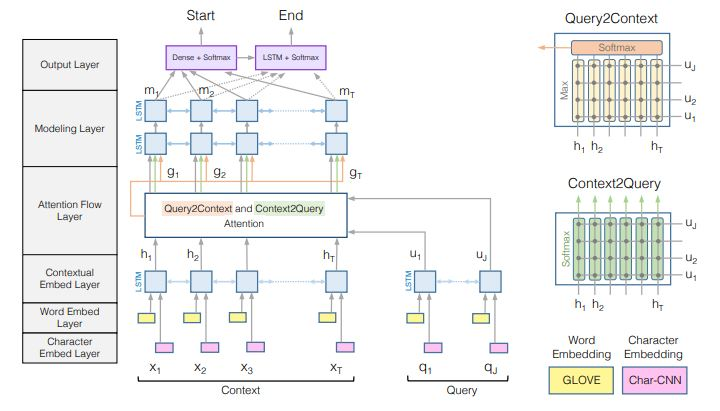
\includegraphics[width=\textwidth,height=8cm]{bidaf_architecture.JPG}
  \caption{Bi-directional attention flow network architecture}
\end{figure*}


The implementation of Bi-directional attention flow networks we utilize  \cite{bidaf:2017} is specially designed for datasets where the anwer $A$ is a sub string of the passage $P$. This is clearly reflected in the architecture of the network, where the inputs are the context passage and the query, and output are basically two integers, indicating the start and end indices of the answer text within the context query. To achieve this, the training loss to be minimized can be expressed as the sum of the negative log probabilities of the true start and end indices by the predicted distributions, averaged over all examples:

$$
L(\theta)  = - \frac{1}{N} \sum^N_i log(p^1_{y^1_i}) + log(p^2_{y^2_i})
$$

where $\theta$ is the set of all trainable weights in the model including CNN filters and LSTM cells, $N$ is the number of train examples and $y_1_i$ and $y_2_i$ are the true start and end indices of the \textit{i}-th example respectively and $p_k$ indicates the \textit{k}-th value of the vector $p$, which represents the probability distributions of the start and end indices over the entire paragraphs, and is obtained form the softmax calculation in the output layer \cite{bidaf:2017}.

%\centering
%

\subsection{Transfer learning}
\label{ssec:transfer_learning}
Here we provide useful definitions and conventions related to transfer learning. Let a domain  $\textbf{D}$ consist of a feature space $\textbf{X}$ and a marfinal probability distribution $P(X)$. Given a source domain $\textbf{D}_s$ and a learning task $\textbf{T}_s$, a target domain $\textbf{D}_t$ and a target task $\textbf{T}_t$, \textit{trasnfer learning} aims to improve the learning of the predictive function for $\textbf{D}_t$ using the knowledge in $\textbf{D}_s$ and $\textbf{T}_s$. In the \textit{inductive transfer learning} setting, the target task is different from the source task, no matter when the source and target domains are the same of not. Conversely, in \textit{transductive transfer learning}, the source and target tasks are the same, while the domains are different. In this situation, little or no labeled data are available in the target domain, while lots of data are present for the source domain \cite{surveytransferlearning} \cite{conneau:2017} \cite{deepcontextualizedwr} \cite{conneau:2017}. 

In computer vision, neural network models are rarely trained from scratch. In general, initial weights are the result of training with ImageNet \cite{imagenet}, a large-scale hierarchical image database, to obtain features. There is already relevant work studying transfer learning over text tasks, mostly around vector representations of words. 

\section{Methods}
\label{sec:methods}

In this section, we describe our methods to study transfer learning over BiDAF networks. 

First, we train a BiDAF network on the SQuAD dataset, being this our source task and domain, and we'll refer to the resulting model as the \textit{source model}. Since we want to study how we can transfer the knowledge to other tasks and domains with none or limited labeled data, we perform a number of transfer experiments with varying amounts of labeled question-answer pairs from the MS-MARCO dataset, which will be our target task and domain for transfer learning.

Let $n$ be the number of labeled samples in the target domain we want to experiment with, then an experiment is as follows: Select $n$ random question-answer pairs from the MS-MARCO dataset, re-train the source model on the randomly selected pairs, and evaluate the resulting model on the MS-MARCO evaluation set. We run this experiment multiple times, for different values of $n$, including $n=0$, which is the case where the target domain has $0$ labeled examples. 

Finally, we also train another BiDAF network on the MS-MARCO dataset without transfer, as a goal for accuracy. The ideal result of this experiment is to achieve similar accuracy in our transfer experiments as in this non-transfer model, which would mean that we can perform this task successfully without fully training our model for this task. It is worth noting that BiDAF performance over MS-MARCO was never studied, so that is an unexpected contribution of our work, in addition to its main focus around transfer learning.

\section{Results}
\label{sec:results}

\subsection{Bi-DAF over SQuAD dataset}

The first step of our research is to train a BiDAF over the SQuAD dataset. We train for 16.4 hours using a single NVidia K80 GPU, and obtain results very close to those reported in the original study \cite{bidaf:2017}, with exact match percentage of $65.64$ and F1 score of $75.68$. The baseline logistic regression performance for this dataset is exact match percentage of $40.0$ and F1 score of $51$. Human performance for this task is EM at $82.3$ and F1 score of $91.2$ \cite{squad:2016} \cite{rnet}.

\begin{table}[t!]
\begin{center}
\begin{tabular}{l|r|r}
\hline \bf Model & \bf EM & \bf F1 \\ \hline
Logistic regression baseline  \cite{squad:2016} & 40.4 & 51.0 \\
Bi-DAF (Original paper) & 68.0 & 77.3 \\
Bi-DAF (Our result - initial learning rate: 0.8) & 75.68 & \\
Bi-DAF (Our result - initial learning rate: 0.5) & 74.07 & \\
R-Net (Single model) & 76.461 & 84.265 \\
Human performance \cite{squad:2016} & 82.304 & 91.221 \\
\end{tabular}
\end{center}
\caption{\label{squad-table} Results over the SQuAD dataset, including our results, baseline, human performance and state of the art as of the time of writing this work. All results are for single model, ensembles tend to do quite better but add complexity to the study.}
\end{table}

Note that as most literature around this style of machine comprehension, we report EM which represents the percentage of exact matches, and the F1 score, which measures the weighted average of the precision and recall rate at a character level.

\subsection{Bi-DAF over MS-MARCO dataset}

We start by obtaining 500 labeled examples from the MS-MARCO dataset for training and 250 for testing, all in which the answer is a substring of the context passage. We restrict the number of samples, since the purpose of this study is to understand the applicability of architectures such as Bi-DAF to other domains where we have little to no labeled data.

Once we have the labeled samples from MS-MARCO, we run 2 families of experiments: first, we study direct training a new Bi-DAF over that data and second, we study fine tunning Bi-DAF entworks pre-trained over SQuAD dataset with two different learning rates.

For the first experiment, we train a Bi-DAF from scratch over the MS-MARCO 500 labeled samples with no transfer. Given the little amount of data, we expect poor results, but this allows us to compare with the results we'll obtain later from transfer learning, and emphathise the value of knowledge transfer. Many studies on transfer learning start by using direct training transfer path as a baseline or means of comparison \cite{conneau:2017}.

For the second set of experiments, we start with two Bi-DAF networks trained with the SQuAD dataset, using initial learning rates of $0.8$ and $0.5$ respectively. The motivation for this, is that even though the lower learning rate is suboptimal when verifying for SQuAD, it might help to avoid overfitting to the SQuAD domain, and allow for better adaption of the network to the MS-MARCO content. Before fine tuning the network with our MS-MARCO samples, we evaluate the SQuAD trained network over the MS-MARCO evaluation set, to also understand how much the fine tuning does later on. We incrementally fine-tune the pre-trained model with different amount of samples until we reach the total of 500 training samples, and evaluate against our MS-MARCO training samples at each step, to understand the impact of the number of samples used for fine tuning in the transfer performance. 

The results over the MS-MARCO evaluation is depicted in the table below.

\begin{table}[t!]
\begin{center}
\begin{tabular}{l|r|r}
\hline \bf Model & \bf F1 (learning rate = 0.8) & \bf F1 (learning rate = 0.5) \\ \hline
Bi-DAF over MS-MARCO baseline (Direct training - no transfer) & 11.02 & n/a  \\
Bi-DAF SQuAD pre-trained (direct evaluation - no transfer) &  50.97 & 48.33 \\
Bi-DAF SQuAD pre-trained + MS-MARCO fine tuning (133 samples) & 54.88 & 55.02 \\
Bi-DAF SQuAD pre-trained + MS-MARCO fine tuning (250 samples) & 55.71 & 56.83 \\
Bi-DAF SQuAD pre-trained + MS-MARCO fine tuning (500 samples) & 56.01 & \textbf(59.14) \\
\end{tabular}
\end{center}
\caption{\label{squad-table} Results for transfer learning to the MS-MARCO domain, including the no-transfer baseline and the no fine tuning baseline.
\end{table}


\section{Analysis}
\label{sec:analysis}

\subsection {Transfer Learning value}

There are many interesting things exposed by the results. First, the low performance when directly training Bi-DAF network over a dataset with a low number of samples is evident as we obtained an F1 score of $11.02$. This highlights the need for transfer learning towards other domains, since we can't generally obtain domain-specific and rich datasets such as SQuAD. Second, the substantial progress that can be achieved over a bit of fine tuning using a handful of domain-specific samples. With only 500 samples for fine tuning, we increased the F1 score more than 10 percent. This supports the theory in the near future, the SQuAD could be a staple dataset for neural model priming prior to transfer learning, such as ImageNet is in the field computer vision.

It is also worth noting that even though pre-training the model with lower learning rate resulted in worst performance over SQuAD, when applied to transfer learning showed better results, likely because this allowed the network to generalize and perform better when being re-trained and subsequently shown passages and queries from a different domain.

\subsection {Error Analysis}

Of course, an F1 score of $59.14$ is still somewhat low and needs to be improved prior to start applying it in concrete technology. We now evaluate error areas to understand where we are failing, and identify areas for future research. We analyzed the errors for the most accurate model: Bi-DAF SQuAD pre-trained + MS-MARCO fine tuning (500 samples) with initial learning rate of 0.5. Still, F1 scores like these were the state of the art for SQuAD a when it was released, so it is still a great achievement given that we are talking about accuracy on a 500 sample dataset.

Now, we analyze the impact of the kind of answer for evaluating question performance. In the MS-MARCO subset que utilized, we had most of the questions being of numeric answer ($28.4\%$, description answer ($52.6\%$) and location answer (5.7\%). We suspected that there might be specific types of questions where we underperformed, but that was not the case. The within-category F1 scores were never more than 3\% apart from each other.

Analyzing the failing questions, we found 3 specific predominant traits: The formality and correctness of the language, the type of question (Why, when, what, etc) and whether the question has or not an answer.

First, most of the wrongly answered questions had informal writing that would never be in wikipedia, such as text from social networks or specific informal news. 

Second, we observe similar accuracies and F1 scores for questions that started with \textit{Where} and \textit{What} for example ($F1=62.02$ and $F1=61.875$ respectively), but a notorious decrease in performance for \textit{Why} questions ($F1 = 51.105$). The Bi-DAF original authors also report low performance in \textit{Why} and \textit{Where} questions, so we think this might be part of the nature of the architecture, given that these types of questions are as common as the other types in the original dataset, but it needs to be subjected to further analysis.


Finally, we observe very low F1 scores for questions that do not have an answer ($F1 = 0.48.12$), which means that our tended to provide an incorrect answer rather than predict that there was no answer. However, in our 500 samples dataset, there were only two such questions, so this low perofrmance might be related to imbalances in our training set and underlying dataset.


\section{Future work}
\label{sec:next_steps}

Overall, the goals following this study center around improving the performance of transfer learning to reach performances that allow the direct applicability of these concepts to technology. Below we mention some potential research directions.

First, as a direct continuation of this study, we will run multiple experiments to compensate for the issues found in the error analysis, such as questions without answers, \textit{why} questions, etc.

Additionally, other model-specific techniques should be studied, such as a broader range of learning rates for the pre-training over the SQuAD dataset. Another experiment to consider would be to not freeze the embedding layer after completing the SQuAD training, and rather keep training embeddings during fine tuning.

Another crucial direction would be to now apply this over the top performing ensembles. For simplicity, we did this study over Bi-DAF which achieves $F1 = 77.3$ over SQuAD. However, there are Bi-DAF based ensembles from the same authors in the leaderboard that achieve much higher results, such as the recent BiDAF + Self Attention + ELMo (ensemble) which obtained $F1 = 87.432$, and is currently in the 5th position in the SQuAD leaderbord. Should that performance improvement translate into our transfer experiments, we would be already obtaining a substantial increase in the overall applicability of this approach.


% include your own bib file like this:
%\bibliographystyle{acl}
%\bibliography{acl2018}
\bibliography{acl2018}
\bibliographystyle{acl_natbib}



\end{document}
